%!TEX root = report.tex
\exercise{Global thresholding}
\subsection{\texttt{IPautothres}}
Global thresholding is a method to extract one or several different object(s) from an image. 
In the most basic case a foreground object of interest is separated from the background, but it can be expanded to more complex segmentations. 
One obvious way to extract objects from the background is by selecting a threshold \(T\) and classify a pixel to a category based on the intensity of that pixel with respect to the threshold\footnote{insert citation to book here}. 
Mathematically speaking, a pixel in a segmented pixel, \(g(x, y)\) is given by 
\[ 
  g(x,y) = \left\{ 
  \begin{array}{l l}
    1 & \quad \text{if \(f(x, y) > T\)}\\
    0 & \quad \text{if \(f(x, y) \leq T\)}
  \end{array} \right.
\]
If \(T\) is constant throughout the image this operation is global thresholding.

One obvious problem with this method is choosing the best value of \(T\) which optimally separates an object from the background. 
The notion of global autothresholding rests on that the mean intensity values between the segmented groups should be close to each other.

The estimation of \(T_a\) can be done in an iterative manner. 
An initial estimate \(T_0\) is made and an image is segmented using this threshold. 
The means \(m_1, m_2\) are calculated of both segmented groups.
Then the next value is calculated using \(T_{n+1} = \frac{m_1 + m_2}{2}\).
This process is repeated until an optimal value \(T_a\) is reached. 
This optimal value is reached when \(\abs{T_n - T_{n - 1}} < \Delta T\) for some predefined precision \(\Delta T\).
\clearpage
We have implemented this algorithm in the function \texttt{IPautothres}:
\matlabexternal{../IPautothresh.m}

As the code displays we set the value of \(T_i\) to the middle value of the image. 
We found that this provides an adequate initial guess in most cases and is therefore warranted. 

\subsection{All Around the World or the Myth of Fingerprints}
We have tested the function on the image \texttt{fingerprint.tif} with \(\Delta T = \frac{1}{10}\). 
This figure is displayed in figure~\ref{fig:original_fingerprint} and its segmentation is visible in figure~\ref{fig:segmented_fingerprint}.
The value of \(T_i = 97.5\) and the reported value of \(T_n = 125.386\) which is close to the literature value of 125.
As visible with the naked eye, figure~\ref{fig:segmented_fingerprint} seems be a good segmentation of figure~\ref{fig:original_fingerprint}.
\begin{figure}[htb]
 \centering
 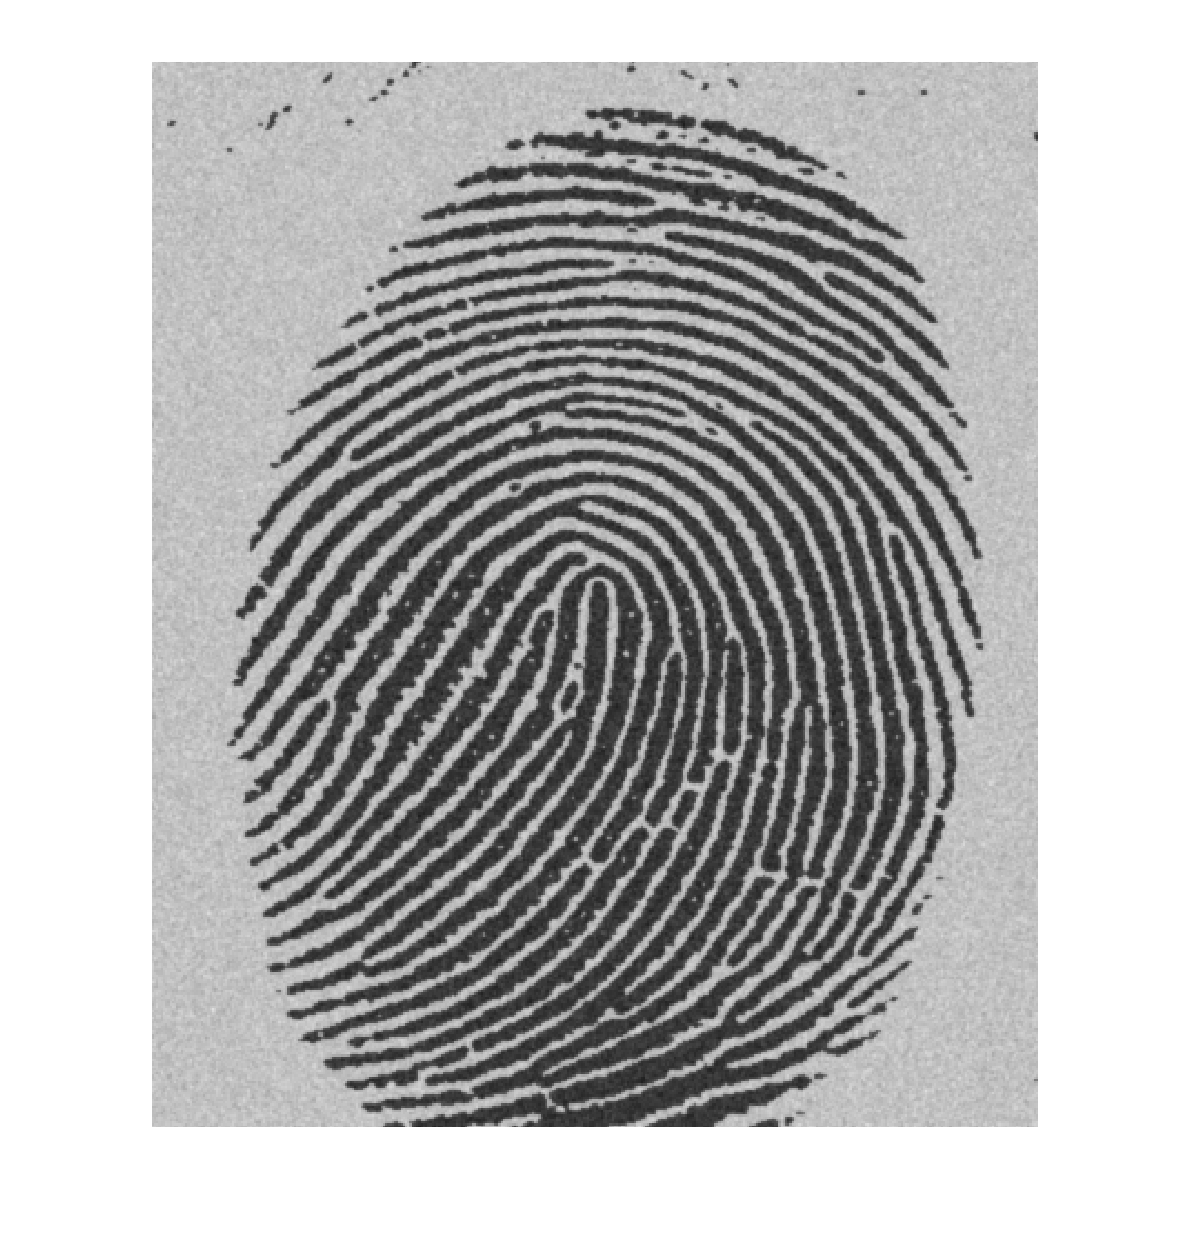
\includegraphics[width=\linewidth]{original_fingerprint.eps}
 \caption{The original fingerprint image}
 \label{fig:original_fingerprint}
\end{figure}

\begin{figure}[htb]
 \centering
 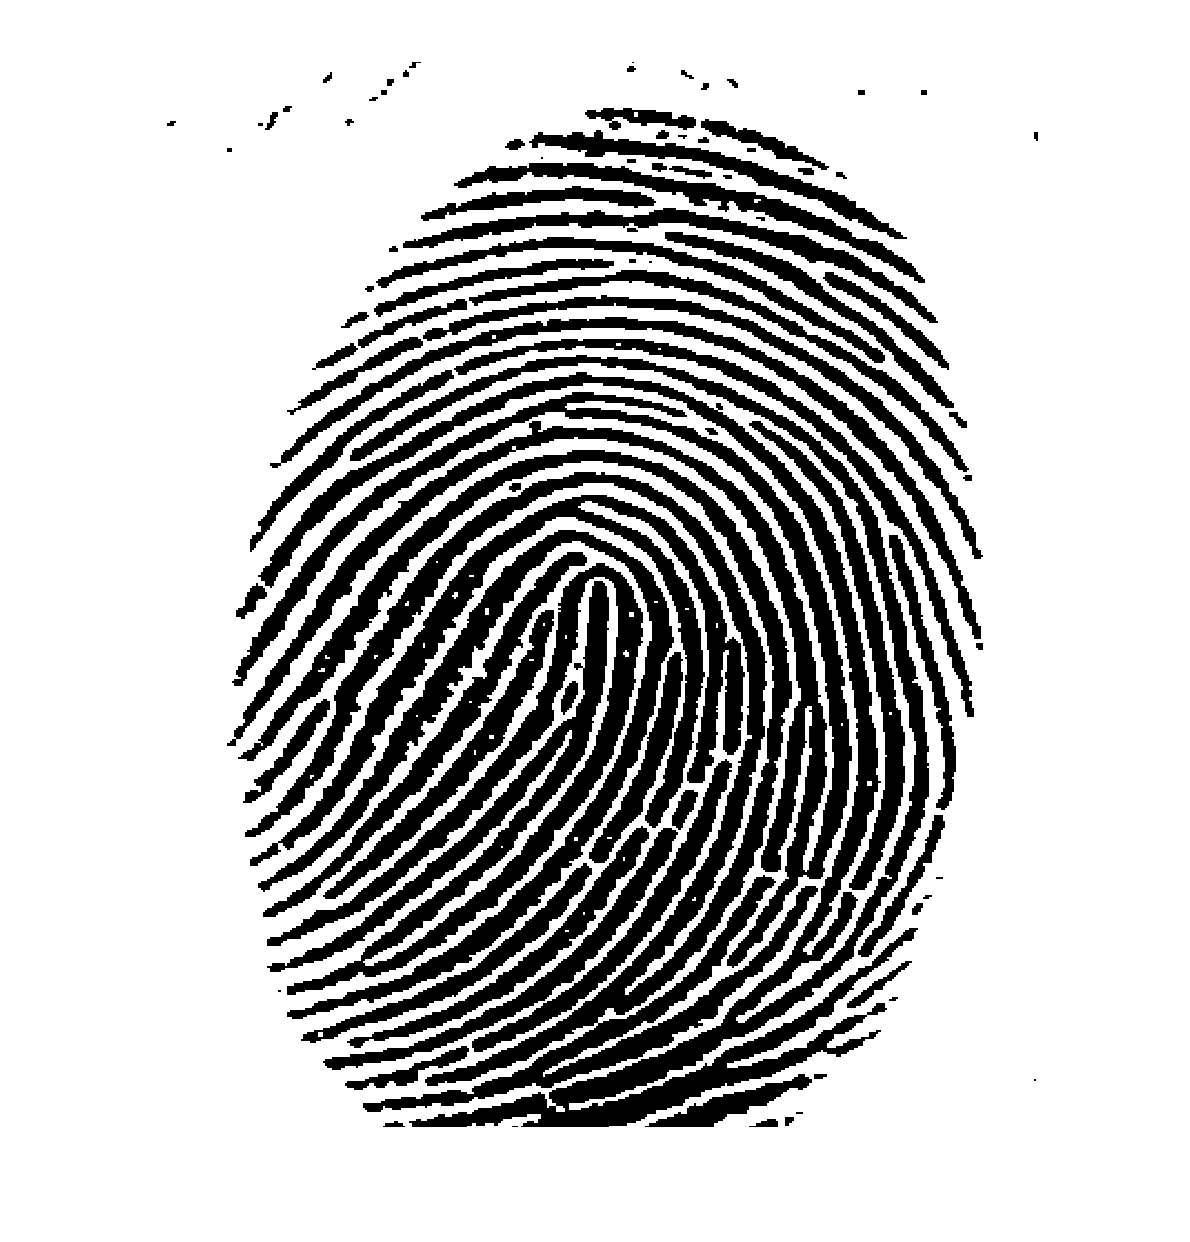
\includegraphics[width=\linewidth]{segmented_fingerprint.eps}
 \caption{The thresholded fingerprint image}
 \label{fig:segmented_fingerprint}
\end{figure}
\clearpage